% Drawing 148/01-2 -- folder 148, batch 01, archive page 6 (PDF page 7).
% Transcription: à gauche, un croquis : un carré hachuré découpé en quatre, sommets $e$, $\eta'$, $\eta''$, $\eta$
% Kind: hatched square cut in four. Method 2 (schematic redraw from the facsimile). Status: ok.
% Notes: A square cut in four by its medians, the quarters hatched, vertex labels e (bottom left), eta' (left), eta'' (below), eta (inside, right of centre, as read); around it faint pencil strokes of a larger tilted square.
% Coordinates: 1 unit = 1 mm = 1/100 of the crop width (bbox in page fractions: [0.08, 0.48, 0.35, 0.64]).
% Redrawn by Claude (claude-opus-5-5), issue #73, 2026-11-07; not checked by a human; not compiled (no TeX in the session).
% Rights: reproduces part of the work -- behind RENDER_TRANSCRIPTS, never published by itself.
\documentclass[tikz,border=3pt]{standalone}
\usepackage{amsmath,amssymb}
\usetikzlibrary{patterns,arrows.meta}
\tikzset{pencil/.style={black!45}, struck/.style={black!35}, mark/.style={circle,draw,inner sep=1.3pt}, pt/.style={circle,fill,inner sep=0.9pt}, opt/.style={circle,draw,fill=white,inner sep=1.1pt}}
\begin{document}
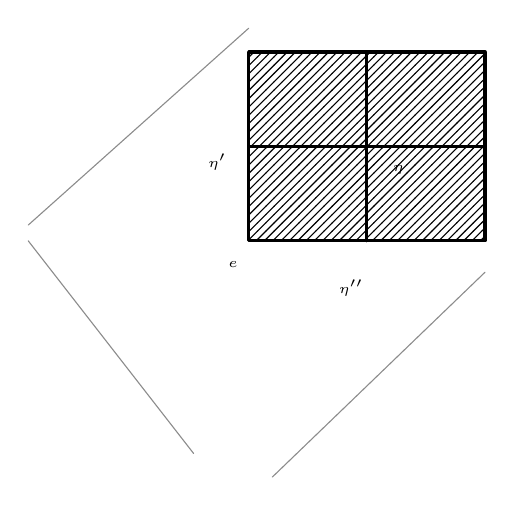
\begin{tikzpicture}[x=1mm,y=1mm,line cap=round,line join=round,font=\scriptsize]
\draw[very thick] (40,-18) -- (70,-18) -- (70,-42) -- (40,-42) -- cycle;
\draw[very thick] (55,-18) -- (55,-42);
\draw[very thick] (40,-30) -- (70,-30);
\fill[pattern=north east lines] (40,-18) -- (55,-18) -- (55,-30) -- (40,-30) -- cycle;
\fill[pattern=north east lines] (55,-18) -- (70,-18) -- (70,-30) -- (55,-30) -- cycle;
\fill[pattern=north east lines] (40,-30) -- (55,-30) -- (55,-42) -- (40,-42) -- cycle;
\fill[pattern=north east lines] (55,-30) -- (70,-30) -- (70,-42) -- (55,-42) -- cycle;
\node[inner sep=1pt] at (38,-45) {\tiny $e$};
\node[inner sep=1pt] at (36,-32) {\tiny $\eta'$};
\node[inner sep=1pt] at (53,-48) {\tiny $\eta''$};
\node[inner sep=1pt] at (59,-33) {\tiny $\eta$};
\draw[pencil] (12,-40) -- (40,-15);
\draw[pencil] (12,-42) -- (33,-69);
\draw[pencil] (43,-72) -- (70,-46);
\end{tikzpicture}
\end{document}
